
\documentclass[twocolumn]{article}
\usepackage{mathpazo}
\usepackage{microtype}
\usepackage{times}
\usepackage{titlesec} % 1
\usepackage[colorlinks = true,
            linkcolor = blue,
            urlcolor  = blue,
            citecolor = blue,
            anchorcolor = blue]{hyperref}
%\usepackage{sectsty} % "제 1 절" ...

 %%%%%%%%%%%%%%%%%%%%%%%%%%%%%%%%%%%%%%%%%%%%%%%%%%%%%%%%%%%%%%%%%%%%%%%%%%%%%
 %                              My Commands
\newcommand{\bi}{\begin{itemize}}
\newcommand{\ei}{\end{itemize}}
\newcommand{\be}{\begin{enumerate}}
\newcommand{\ee}{\end{enumerate}}
\newcommand{\ii}{\item}
\newtheorem{Def}{Definition}
\newtheorem{Lem}{Lemma}

%\usepackage{algorithm}
%\usepackage{algorithmicx}
%\usepackage{algpseudocode}

\usepackage{algpseudocode,algorithm,algorithmicx}
\newcommand*\DNA{\textsc{dna}}

\newcommand*\Let[2]{\State #1 $\gets$ #2}
\algrenewcommand\algorithmicrequire{\textbf{Input:}}
\algrenewcommand\algorithmicensure{\textbf{Output:}}


\usepackage{graphicx}
\graphicspath{%
        {converted_graphics/}
        {./images/}
}

\usepackage{color}
\usepackage{xcolor}
\usepackage{listings}
\usepackage{caption}
\DeclareCaptionFont{white}{\color{white}}
\DeclareCaptionFormat{listing}{\colorbox{gray}{\parbox{\textwidth}{#1#2#3}}}
\captionsetup[lstlisting]{format=listing,labelfont=white,textfont=white}
\usepackage{verbatimbox}

\usepackage[hangul,nonfrench,finemath]{kotex}
    
\setlength\textwidth{7in} 
\setlength\textheight{9.5in} 
\setlength\oddsidemargin{-0.25in} 
\setlength\topmargin{-0.25in} 
\setlength\headheight{0in} 
\setlength\headsep{0in} 
%\setlength\columnsep{5pt}
\sloppy 
 
\begin{document}

\title{
\vspace{-0.5in}\rule{\textwidth}{2pt}
\begin{tabular}{ll}\begin{minipage}{4.75in}\vspace{6px}
\noindent\large {\it KIWI Project}@Data Management Research Section\\
\vspace{-12px}\\
\noindent\LARGE ETRI\qquad  \large Technical Report 15ZS1410-TR-73
\end{minipage}&\begin{minipage}{2in}\vspace{6px}\small
218 Gajeong-ro, Yuseong-gu\\
Daejeon, 305-700, South Korea\\
http:/$\!$/www.etri.re.kr/\\
http:/$\!$/sungsoo.github.com/\quad 
\end{minipage}\end{tabular}
\rule{\textwidth}{2pt}\vspace{0.25in}
\LARGE \bf 근사 질의 처리 개요 \\
\large Overview of Approximate Query Processing
}

\date{}

\author{
{\bf Sung-Soo Kim}\\
\it{sungsoo@etri.re.kr}
}

\maketitle

\begin{abstract}
빅데이터를 바탕으로하고 있는 비즈니스, 과학, 공학 분야에서 데이터주도(data-driven) 활동들이 데이터 크기와 중요성 측면에서 빠르게 성장해 나가고 있다. 
근사 질의처리(approximate query processing)란 데이터베이스에 존재하는 데이터 값들의 샘플링, 히스토그램 또는 웨이블릿 등을 이용하여 사용자가 요구한 정확한 답뿐 아니라 그와 유사한 답까지 제공해 줄 수 있는 질의처리를 의미한다. 
샘플링(sampling)은 빅데이터에 대한 적시 비용-효과적인 분석결과를 얻기 위해 근사 질의처리에서 가장 일반적으로 사용하는 방법 중 하나다.

KIWI 플랫폼의 질의 처리에 필요한 내부 성능 개선을 위해 근사 질의처리 접근법을 고려하고 있다. 
이와 관련하여 본 기술문서에서는 근사 질의처리 배경, 접근방법, 근사 질의처리를 이용하는 주요 응용들을 소개한다.
\end{abstract}


%\begin{algorithm}[H]
%  \caption{Counting mismatches between two packed \DNA strings 
%  \label{alg:packed-dna-hamming}}
%  \begin{algorithmic}[1]
%    \Require{$x$ and $y$ are packed \DNA strings of equal length $n$}
%    \Ensure{$\delta$ is return value}
%      \Let{$z$}{$x \oplus y$} \Comment{$\oplus$: bitwise exclusive-or}
%      \Let{$\delta$}{$0$}
%      \For{$i \gets 1 \textrm{ to } n$}
%        \If{$z_i \neq 0$}
%          \Let{$\delta$}{$\delta + 1$}
%        \EndIf
%      \EndFor
%      \State \Return{$\delta$}
%  \end{algorithmic}
%\end{algorithm}

%\begin{figure}[htb]
%        \centering
%        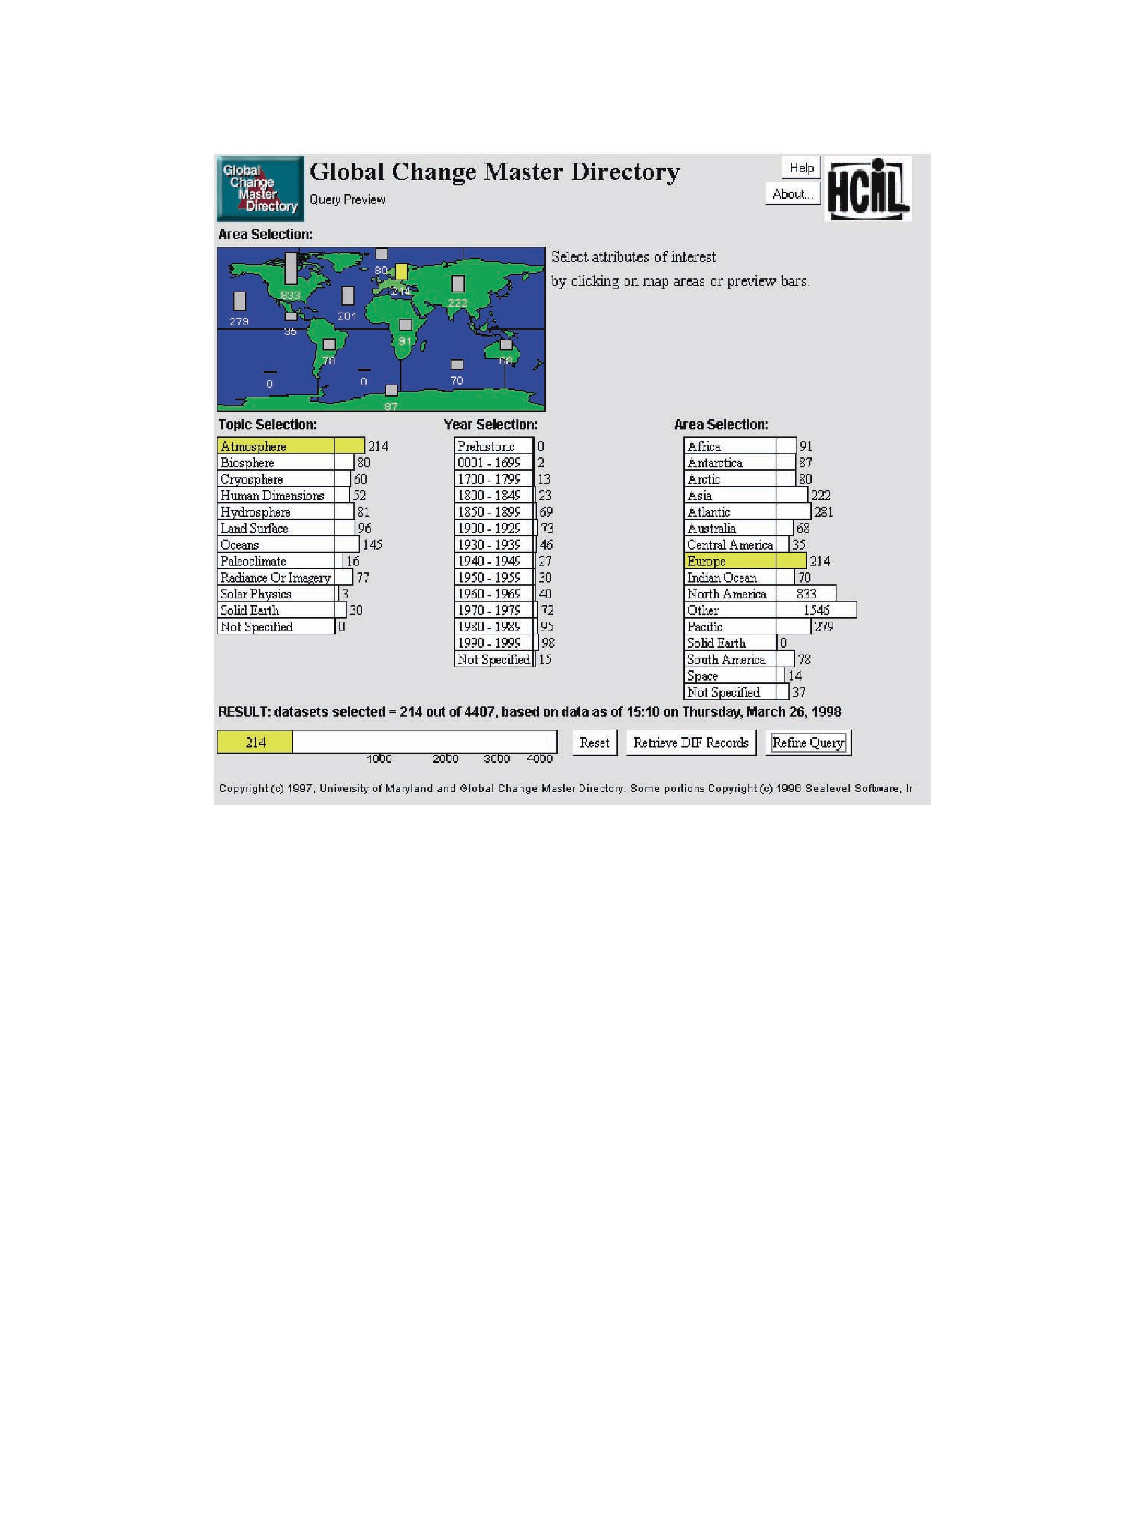
\includegraphics[width=0.48\textwidth]{nasa-gui.pdf}
%        \caption{NASA EOSDIS interface of query preview.}
%        \label{fig:nasa}
%\end{figure}

\section{Introduction}
Query processing in a database context is the process that deduces information that is available in the data- base. Due to the huge amount of data available, one of the main issues of query processing is how to process queries efficiently. In many cases, it is impossible or too expensive for users to get exact answers in the short query response time. \textit{Approximate query processing} (AQP) is an alternative way that returns approximate answer using information which is similar to the one from which the query would be answered. 
It is designed primarily for aggregate queries such as count, sum and avg, etc. 
Given a SQL aggregate query $Q$, the accurate answer is $y$ while the approximate answer is $y'$. 
The relative error of query $Q$ can be quantified as:

\begin{equation}
\textit{Error}(Q) = |\frac{y-y'}{y}|
\end{equation}

The goal of approximate query processing is to provide approximate answers with acceptable accuracy in orders of magnitude less query response time than that for the exact query processing.

\section{Historical Background}
The earliest work on approximate answers to decision support queries appears in Morgenstein’s dissertation from Berkeley \cite{Morgenstein:1981}. 
And the approximate query processing problem has been studied extensively in the last two decades. 
The main motivations \cite{Garofalakis:2001} which drive the techniques being developed are summarized as follows.

First, with the advanced data collection and management technologies, nowadays there are a large number of applications with data sets about gigabytes, terabytes or even petabytes. Such massive data sets necessarily reside on disks or tapes, making even a few accesses of the base data sets comparably slow. 
In many cases, precision to ‘‘last decimal’’ is not required for a query answer. 
Quick approximation with some error guarantee (e.g., the resident population in Australia $21,126,700 \pm 200$) is adequate to provide insights about the data.

Second, decision support system (DSS) and data mining are popular approaches to analyzing large databases for decision making. The main characteristic of the DSS is that aggregation queries (e.g., count, sum, avg, etc.) are executed on large portion of the databases, which can be very expensive and resource intensive even for a single analysis query. Due to the exploratory nature of decision making, iterative process involves multiple query attempts. Approximate answers with fast response time gives users the ability to focus on their explorations and quickly identify truly interesting data. It provides a great scalability of the decision support applications.
\begin{figure}[htb]
        \centering
        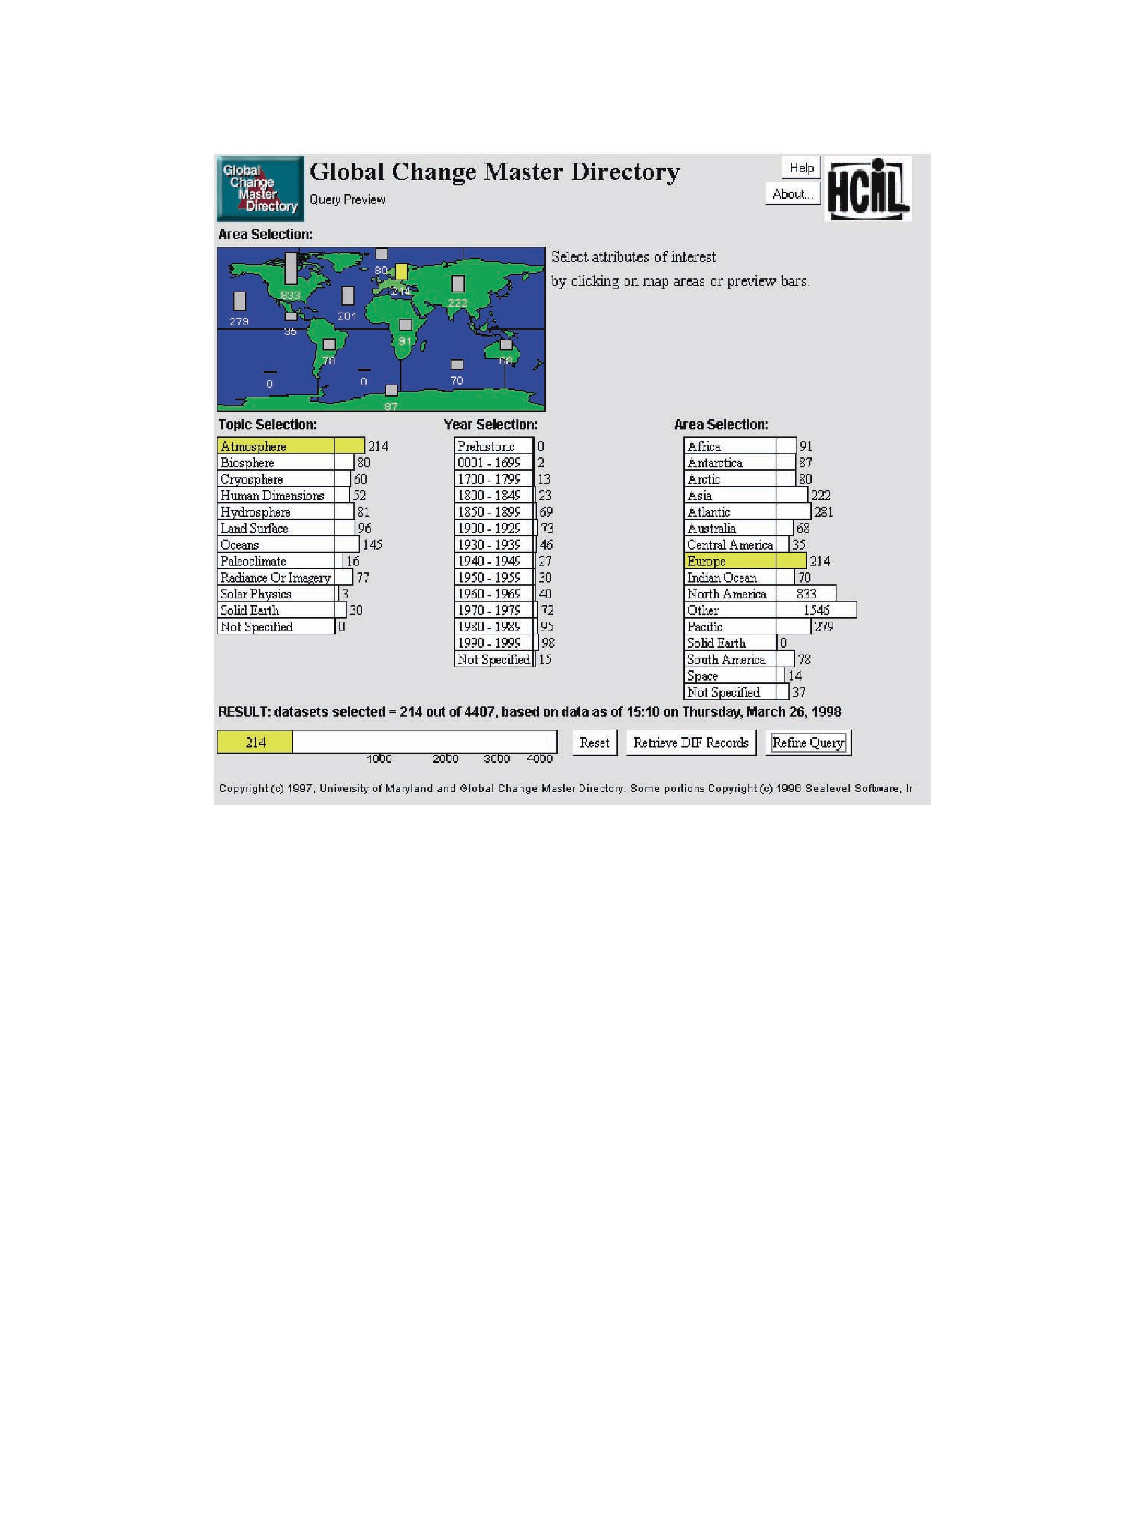
\includegraphics[width=0.48\textwidth]{nasa-gui.pdf}
        \caption{NASA EOSDIS interface of query preview.}
        \label{fig:nasa}
\end{figure}

Third, approximate query processing is also used to provide query preview. In most cases, users are only interested in a subset of the entire database. Given a trial query, query preview provides an overview about the data distribution. The users can preview the number of hits and refine the queries accordingly. This prevents users from fruitless queries such as zero-hits or mega-hits. Figure \ref{fig:nasa} shows an example of query preview interface of NASA EOSDIS (Earth Observing System Data and Information System) project, which is attempting to provide online access to a rapidly growing archive of scientific earth data about the earth’s land, water, and air. In the query preview, users select rough ranges for three attributes: area, topic (a menu list of parameters such as atmosphere, land surface, or oceans) and temporal coverage. The number of data sets for each topic, year, and area is shown on preview bars. The result preview bar, at the bottom of the interface, displays the total approximate number of data sets which satisfy the query.
Finally, sometimes network limitation or disk storage failure would cause the exact answers unaffordable or unavailable. An alternative solution is to provide an approximate answer based on the local cached data synopsis.

\section{Foundations}
Due to the acceptability of approximate answers coupled with the necessity for quick query response time, approximate query processing has emerged as a cost effective approach for dealing with the large amount of data. This speed-up is achieved by answering queries based on samples or other synopses (summary) of data whose size is orders of magnitude smaller than that of the original data sets.
\begin{figure}[htb]
        \centering
        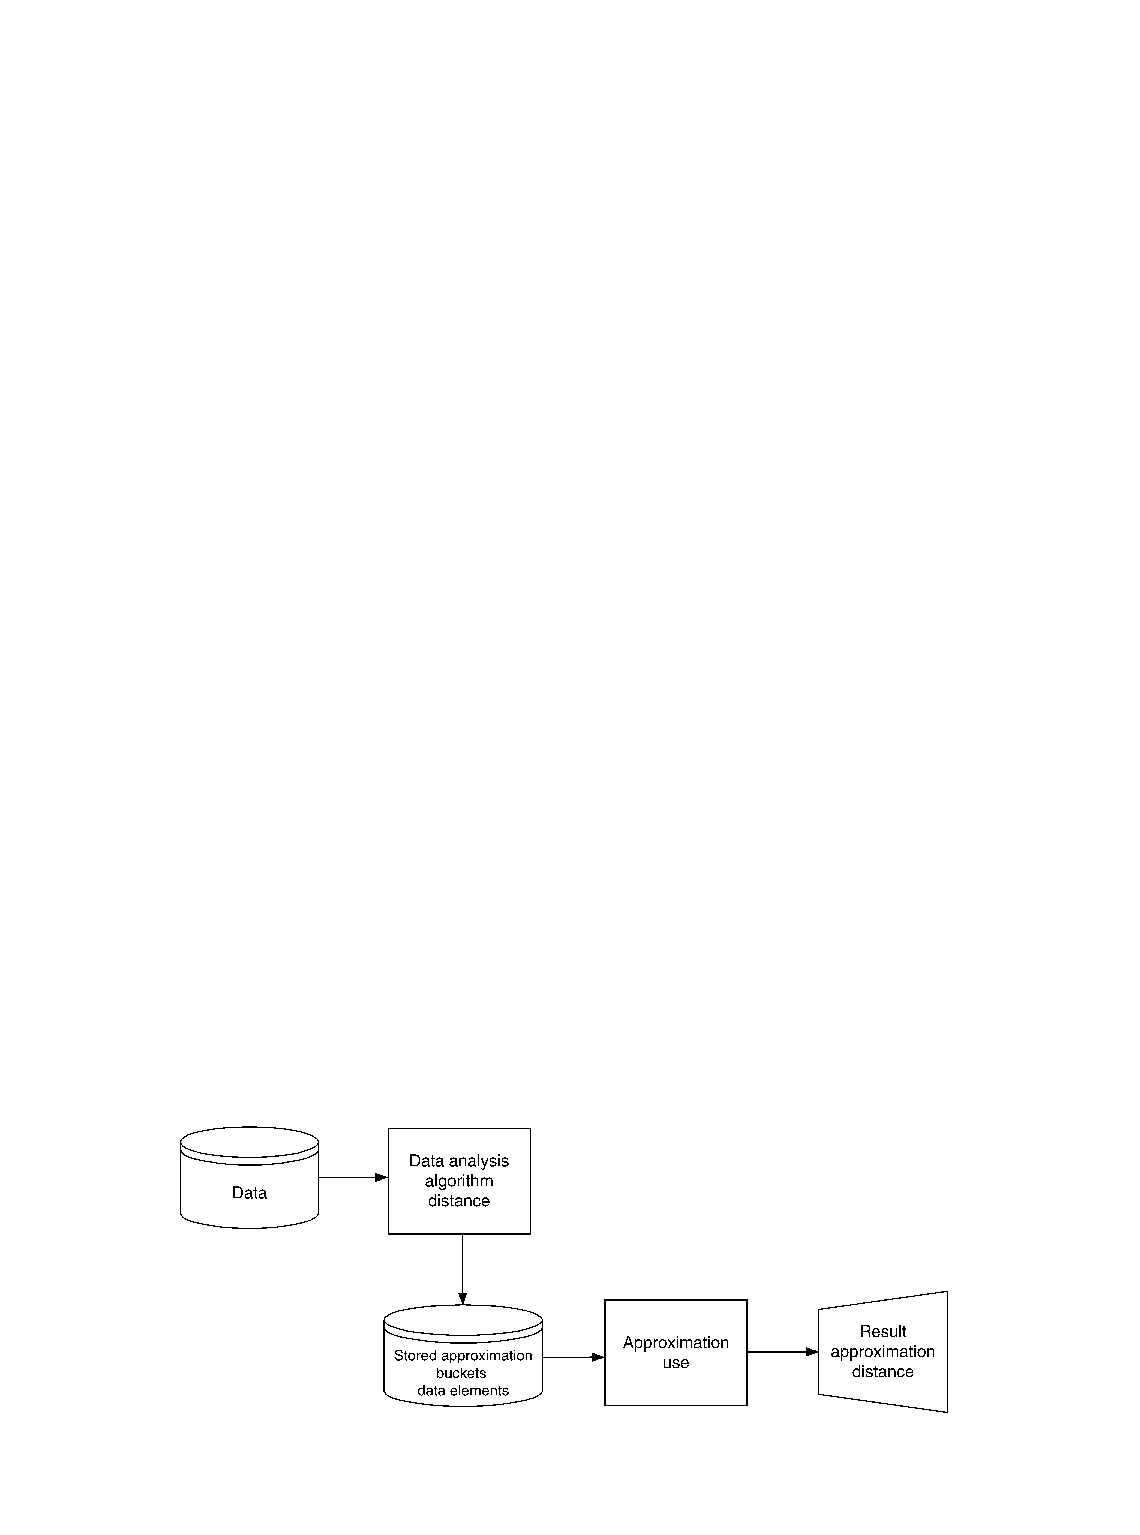
\includegraphics[width=0.48\textwidth]{generic-flow.pdf}
        \caption{Generic flow of approximation process.}
        \label{fig:flow}
\end{figure}

Ioannidis presented the generic flow of approximate query process (Fig. \ref{fig:flow}) in \cite{Ioannidis:2003-b}. Here, data analysis is the overall approach which derives the synopsis from original data to approximate the underlying data distribution. 
Typically, the \textit{algorithm} partitions the data based on the \textit{distance} function into groups of similar elements, called \textit{buckets}, clusters, patterns, or several other names. The \textit{data elements} that fall in each bucket are then represented by the synopses for \textit{approximation use} which corresponds to the actual purpose of the whole data approximation process. The quality of approximation result can be measured by the \textit{distance} between the synopses and the original data.

There are two basic approaches to achieve approximate query processing: pre-computed synopsis and online query processing.

\subsection{Pre-Computed Synopsis}

Approximate query processing using pre-computed synopsis includes two steps: construct synopsis prior to query time, answer query approximately using synopsis at query time.

To provide high accurate query answer, the key issue to construct synopsis is how to represent the underlying data distribution precisely and compactly. Generally, the data distribution can be classified into two groups: uniform distribution and non-uniform distribution. The synopsis for uniform data distribution assumes the objects are distributed uniformly in the data space. For point objects locating in two-dimensional space $[{U^x}_{min}, {U^y}_{min}] \times [{U^x}_{max}, {U^y}_{max}]$, the query result size is estimated as 
$N \times \textit{area}(Q)/(({U^x}_{max} - {U^x}_{min}) \times ({U^y}_{max} - {U^y}_{min}))$, where $N$ is the data set size and $\textit{area}(Q)$ is the area of window query $Q$.

There are various techniques developed for non- uniform data distribution. They can also be divided into two groups: parametric and non-parametric. The parametric techniques try to use parameters to catch the original data distributions. Although the models can summarize data distributions with a few descriptive parameters, if the underlying data do not follow any known distributions, or their linear combinations, the model fitting techniques produce inferior results.

The non-parametric techniques use different approaches to summarize the data distributions. 
Generally, it is possible to classify these techniques into three categories according to the strategies adopted:

\be
\ii Sampling techniques
\ii Histogram techniques
\ii Wavelet techniques
\ee

\subsubsection*{Sampling}
The basic idea of sampling is that a small random sample of the data often well-represent all the data. Therefore, query would be answered based on the pre-sampled small amount of data and then scaled up based on the sample rate. 
Figure \ref{fig:sampling} shows an example where 50\% of data are sampled during the pre-computed stage. 
\begin{figure}[htb]
        \centering
        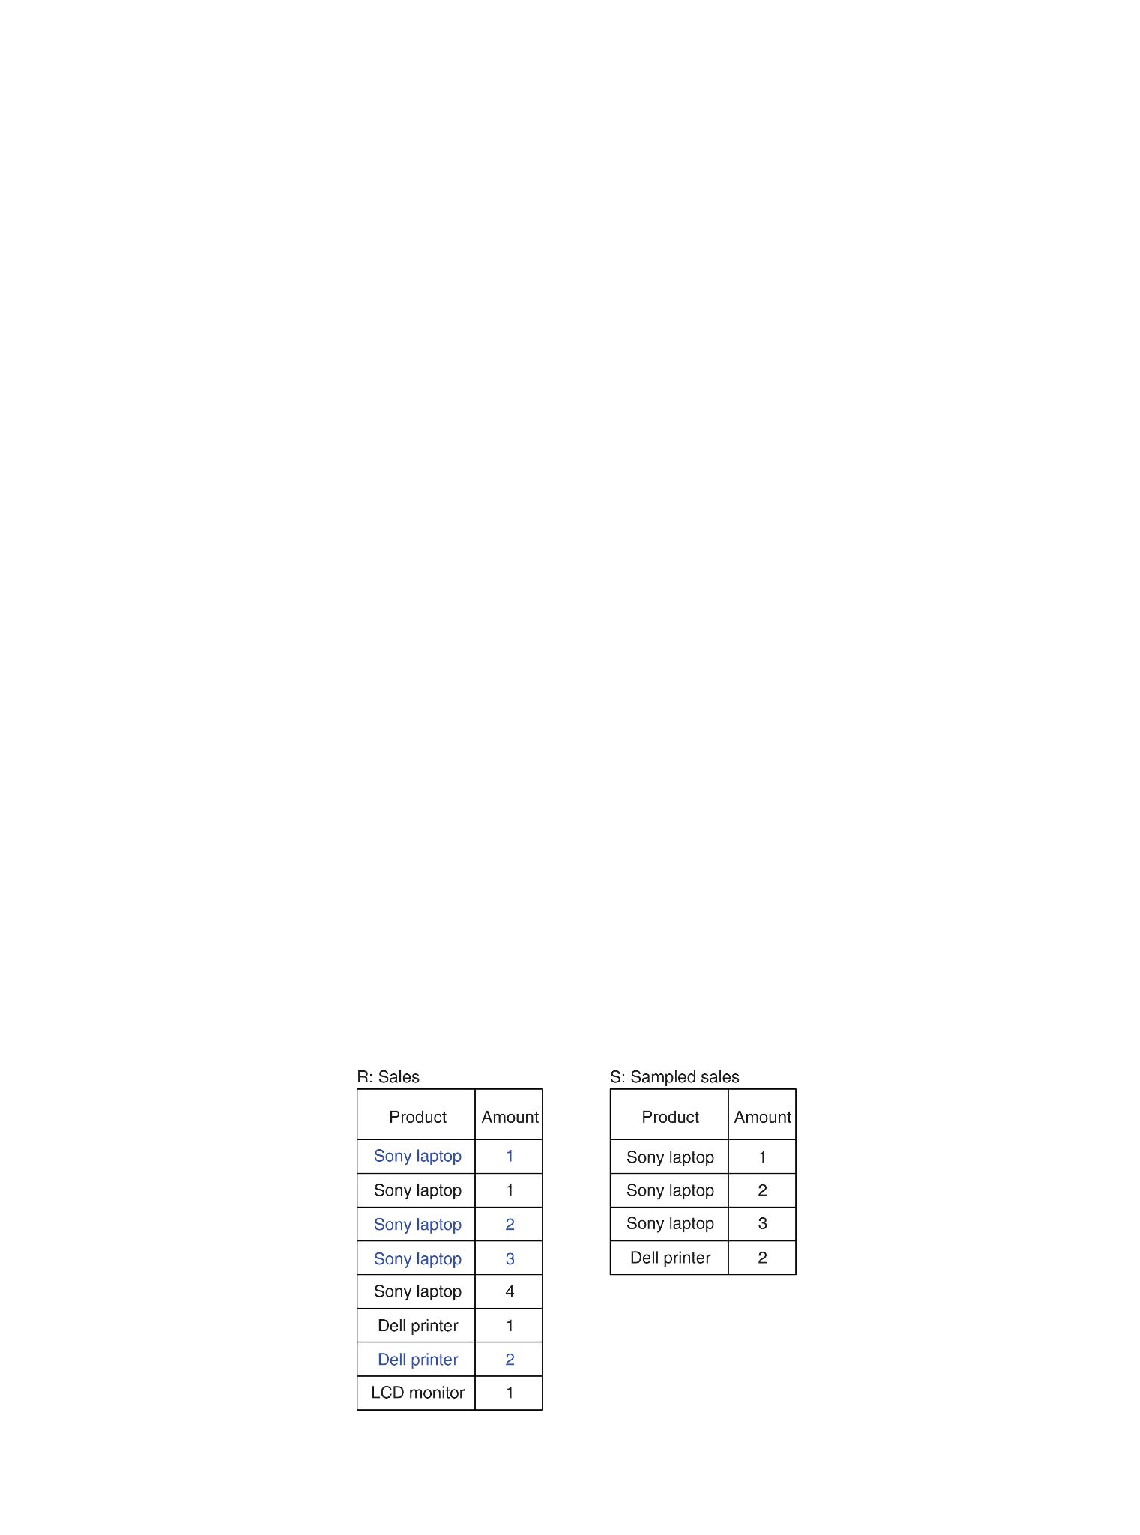
\includegraphics[width=0.48\textwidth]{sampling-example.pdf}
        \caption{Example of sampling.}
        \label{fig:sampling}
\end{figure}

Given a query ‘‘how many Sony laptops are sold in $R$’’, 
the approximate result is ‘‘select 2 * sum(*) from $S$ where $S$.\textit{product} = '\textit{SonyLaptop}'’’, which is 12. In $R$, the exact answer is 11.

The main issue of sampling method is to decide what sample criteria should be used to select data. The
sampling techniques are classified into the following groups \cite{Wang:2008}:

\be
\ii \textit{Uniform sampling}. Data is sampled uniformly
\ii \textit{Biased sampling}. A non-uniform random sample is pre-computed such that parts of the database
deemed ‘‘more important’’ than the rest
\ii \textit{Icicles}. A biased sampling technique that is based on
known workload information
\ii \textit{Outlier indexing.} Indexing outliers and biased sampling the remaining data
\ii \textit{Congressional sampling.} Targeting group by queries
with aggregation and trying to maximize the accuracy for all groups (large or small) in each group-by query
\ii \textit{Stratified sampling.} Generalization of outlier indexing, Icicles and congressional sampling. 
It targets minimizing error in estimation of aggregates for the given workload
\ee

Sample-based procedures are robust in the presence of correlated and nonuniform data. Most importantly, sampling-based procedures permit both assessment and control of estimation errors. The main disadvantage of this approach is the overhead it adds to query optimization. 
Furthermore, join operation could lead to significant quality degradations because join opera- tor applied on two uniform random sample can result in a non-uniform sample of the join result which contains very few tuples.

\subsubsection*{Histograms} 
Histogram techniques are the most commonly used form of statistics in practice (e.g., they are used in DB2, Oracle and Microsoft SQL Server). 
This is because they incur almost no run-time overhead and produce low-error estimates while occupying reasonably small space.
The basic idea is to partition attribute value domain into a set of buckets and query is answered based on the buckets. The main issues of histogram construction and query are as follows:

\bi
\ii How to partition data into bucket
\ii How to represent data in each bucket
\ii How to estimate answer using the histogram
\ei

For one-dimensional space, a histogram on an attribute $X$ is constructed by partitioning the data distribution of $X$ into $B$ ($B \geq 1$) buckets and approximating the frequencies and values in each bucket. 
Figure \ref{fig:histogram}a is an example of original data set and Figure \ref{fig:histogram}b shows its data distribution. 
Figure \ref{fig:histogram}c is an example of histogram constructed accordingly, where $B = 3$.
\begin{figure*}[htb]
        \centering
        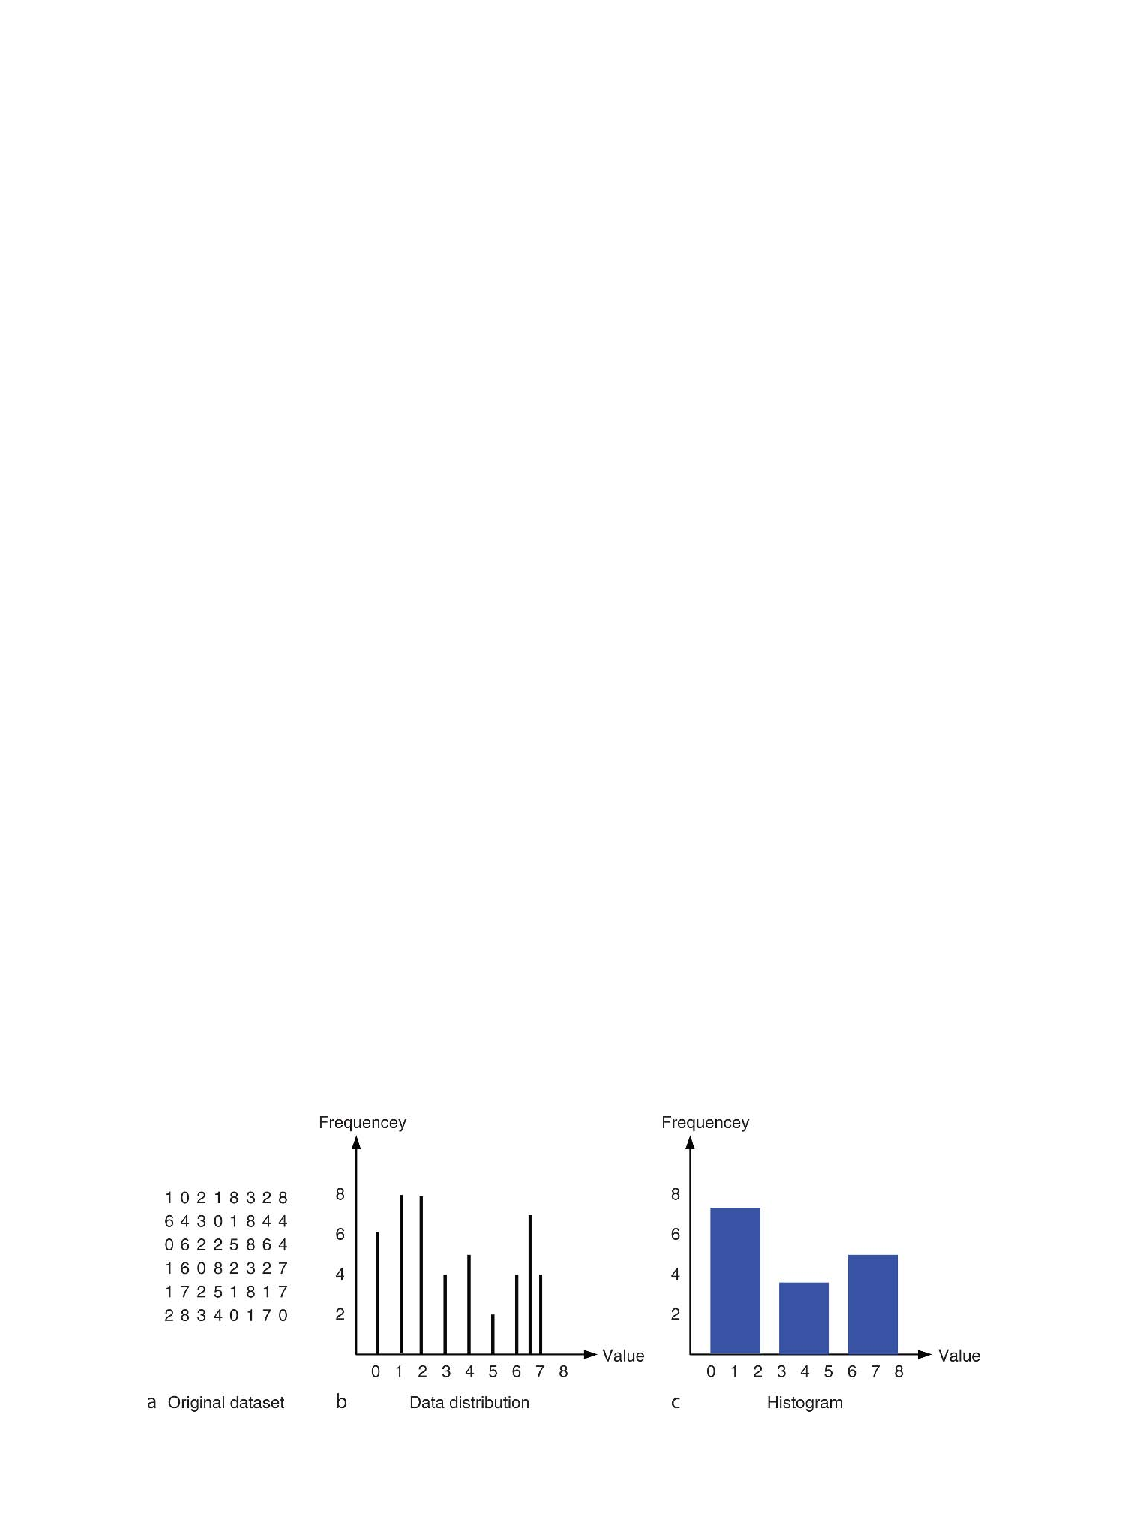
\includegraphics[width=0.8\textwidth]{histogram-example.pdf}
        \caption{Example of histogram.}
        \label{fig:histogram}
\end{figure*}

If there are several attributes involved in a query, a multi-dimensional histogram is needed to approximate the data distribution and answer such a query. A multi-dimensional histogram on a set of attributes is constructed by partitioning the joint data distribution of the attributes. They have the exact same characteristics as one-dimensional histograms, except that the partition rule needs to be more intricate and cannot always be clearly analyzed because there cannot be ordering in multiple dimensions \cite{Poosala:1997}.

To represent data in each bucket, it includes value approximation and frequency approximation. Value approximation captures how attribute values are approximated within a bucket. And frequency approximation captures how frequencies are approximated within a bucket.

The two main approaches for value approximation are \textit{continuous value assumption} and \textit{uniform spread assumption} \cite{Poosala:1996}.
Continuous value assumption only maintains min and max value without indication of how many values there are or where they might be. Under the uniform spread assumption, one also maintain the number of values within each bucket and approximates the actual value set by the set that is formed by (virtually) placing the same number of values at equal distances between the min and max value in multi-dimensional space \cite{Ioannidis:2003}.

With respect to frequency approximation, almost all work deal with uniform distribution assumption.
The benefit of a histogram synopsis is that it can be easily used to answer many query types, including the aggregate and non-aggregate queries. However, one of the issues of histogram approach is it is hard to calculate a theoretical error bound. Thus the evaluations on the histogram synopsis usually rely heavily on the experiment results. Further more, histogram-based approaches become problematic when dealing with the high-dimensional data sets that are typical for modern decision support applications. This is because as the dimensionality of the data increases, both the storage overhead (i.e., number of buckets) and the construction cost of histograms that can achieve reasonable error rates increase in an explosive manner.

\subsubsection*{Wavelet} 
Wavelet is a mathematical tool for hierarchical decomposition of functions using recursive pair- wise averaging and differencing at different resolutions. It represents a function in terms of a coarse overall shape, plus details that range from broad to narrow. It is widely used in the signal and image processing.

Matias et al. \cite{Matias:1998} first proposed the use of Haar-wavelet coefficients as synopsis for estimating the selectivity of window queries. The basic idea is to apply wavelet decomposition to the input data collection to obtain a compact data synopsis that comprises a select small collection of wavelet coefficients. 
Figure \ref{fig:wavelet} shows an example of hierarchical decomposition tree of Haar-wavelet. The leaf nodes are original data and non-leaf nodes are wavelet coefficients generated by averaging and differencing from their two children.
\begin{figure}[htb]
        \centering
        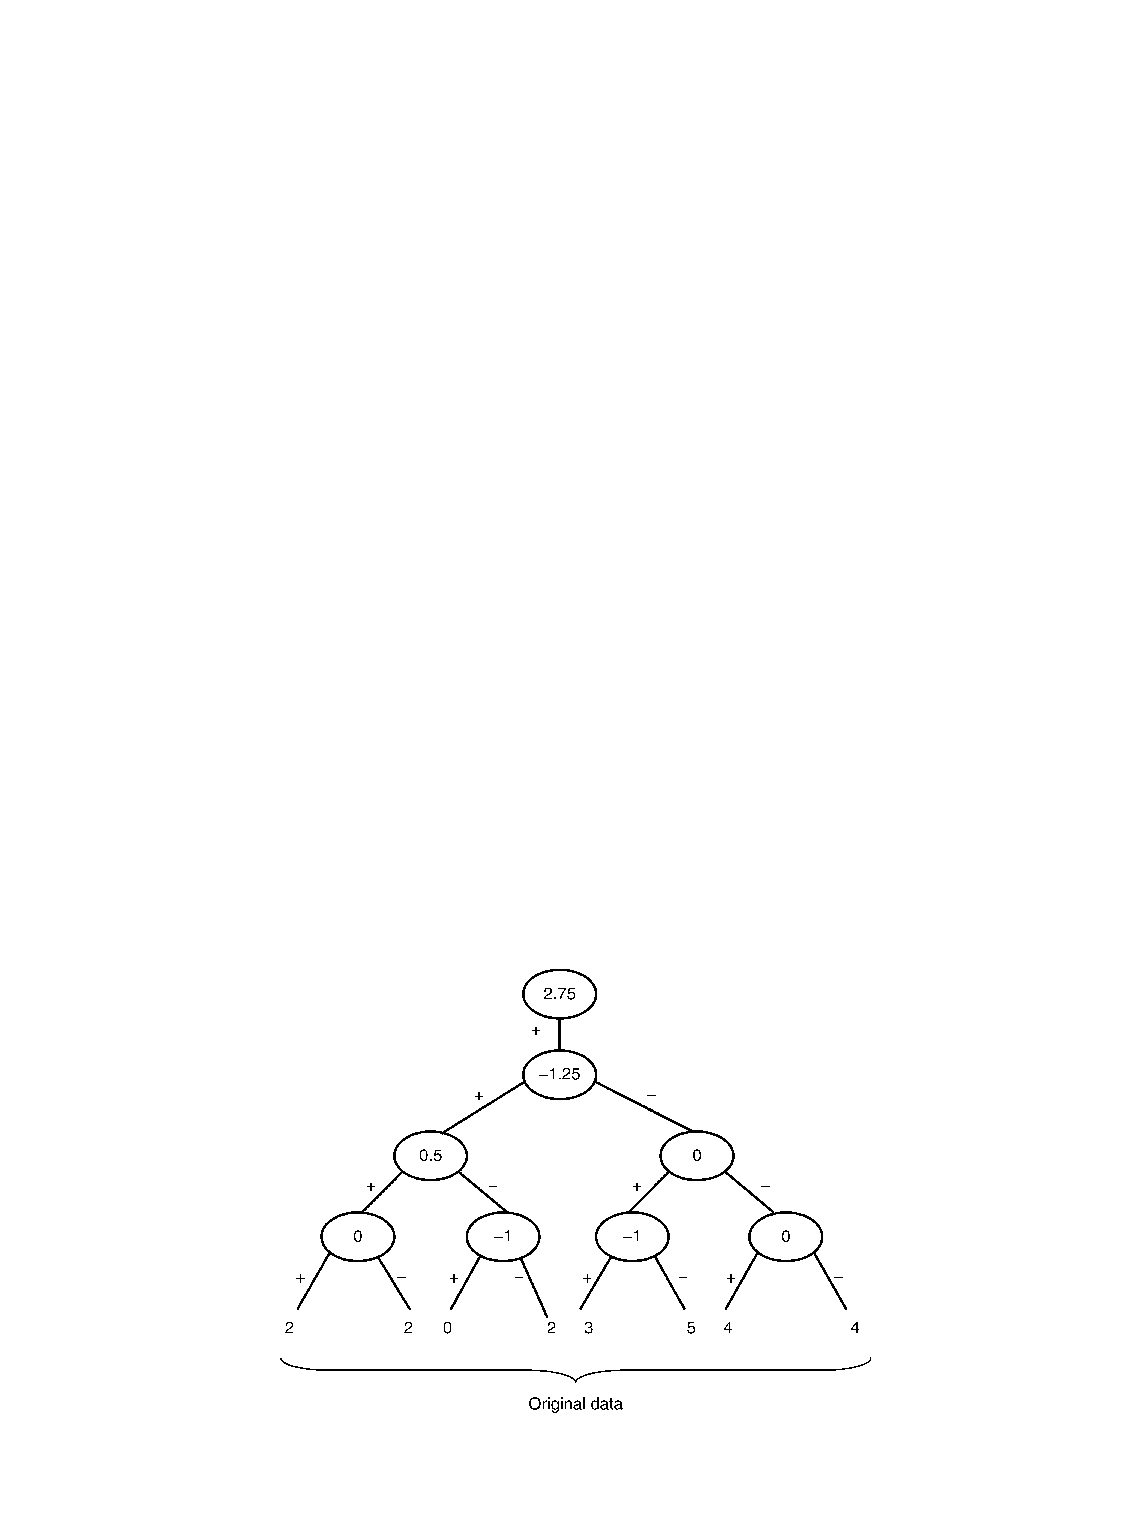
\includegraphics[width=0.48\textwidth]{wavelet-example.pdf}
        \caption{Example of Haar-wavelet hierarchical decomposition.}
        \label{fig:wavelet}
\end{figure}

Later, the wavelet concept was extended to answer more general approximate queries. The results of recent studies have clearly shown that wavelets can be very effective in handling aggregates over high-dimensional online analytical processing (OLAP) cubes, while avoid- ing the high construction costs and storage overheads of histogram techniques.

Another important part of the above three technologies for approximate query processing is synopsis maintenance. If the data distribution is not changed significantly, the data synopsis would be updated accordingly to reflect such change. Otherwise, a new data synopsis will be constructed and discard the old one. Refer to the specific techniques for more details.

There are a few other work that do not belong to the above three categories to approximate the underlying data distribution. 
For example, recently Das et al. \cite{Das:2004} present a framework that is based on randomized projections. This is the first work in the context of spatial database which provides probability quality guarantees with respect to query result size approximation.

\subsection{Online Query Processing}
The motivation of online query processing is that the data analysis is to extract unknown information from data. It is an iterative process starting by asking broad questions and continually refining them based on approximate or partial results. Therefore, instead of optimizing for query response time, it needs to balance two conflicting performance goals: minimizing uneventful ‘‘dead time’’ between updates for the users, while simultaneously maximizing the rate at which partial or approximate answers approach a correct answer. Refer to \cite{Hellerstein:1997} for details.

Compared with pre-computed synopses approach, the advantages of online query processing approach is it does not require pre-processing and progressive refinement of approximate results at runtime can quickly lead to a satisfied results. However, the main obstacles for this technique to be practical is it significantly changes the query processor of current commercial query processing system which is not desirable.



\section{Key Applications}

\subsubsection*{AQP in Relational Data Management}
The AQUA system proposed by the Bell lab can sup- port various kinds of approximate queries over the relational database.

\subsubsection*{AQP in Spatial Data Management}
Alexandria Digital Library allows user to define spatial queries and returns the approximate number of hits quickly as the initial result and then user can refine the query accordingly.

\subsubsection*{AQP in Stream Data Management}
MIT proposed Aurora as a data stream management system, which virtually supports answering approximate queries over the data stream.

\subsubsection*{AQP in Sensor Network}
The techniques of TinyDB system, proposed by Massachusetts Institute of Technology and UC Berkeley, can lead to orders of magnitude improvements in power consumption and increased accuracy of query results over non-acquisitional systems that do not actively control when and where data is collected.

\subsubsection*{AQP in Semantic Web Search}
For semantic web search, the viewpoints of users performing a web search, ontology designers and annotation designers do not match. This leads to missed answers. Research studies have shown AQP is of prime importance for efficiently searching the Se- mantic Web.



\bibliographystyle{abbrv}
\bibliography{sqlonhadoop}

\end{document}
